\chapter{Surfaces, Adsorption and Heterogeneous Catalysis}\label{ch:b3:surfaces-catalysis}

Under a car, inside a steel can, sits a ceramic honeycomb whose thousands of
channels are coated with a porous oxide holding a few grams of platinum,
palladium and rhodium. In a fraction of a second, the exhaust gases flowing
through it lose most of their carbon monoxide, unburnt hydrocarbons and
nitrogen oxides. Nothing happens in the gas: every one of these reactions takes
place on the surface of the metal particles, a few nanometres across. Most of
the chemical industry runs the same way, from the ammonia of fertilisers to
the cracking of petroleum. This chapter describes how molecules stick to
surfaces, how much of a surface they cover, how surface reactions proceed, and
how a solid catalyst is made, measured and looked at.

\begin{recall}
The Year 1 volume defined catalysts and the difference between homogeneous and
heterogeneous catalysis, and described the face-centred cubic packing of
metals. The Year 2 volume defined the conversion, the selectivity and the
turnover frequency of a catalyst, and Le Chatelier's principle.
\Cref{ch:b3:x-ray-diffraction} introduced \omterm{def:b3:x-ray-diffraction:miller}{Miller indices},
\cref{ch:b3:rate-theories} the \omterm{thm:b3:rate-theories:eyring}{Eyring equation} and
\cref{ch:b3:partition-functions} the statistics of distributions.
\end{recall}

\begin{omfigure}
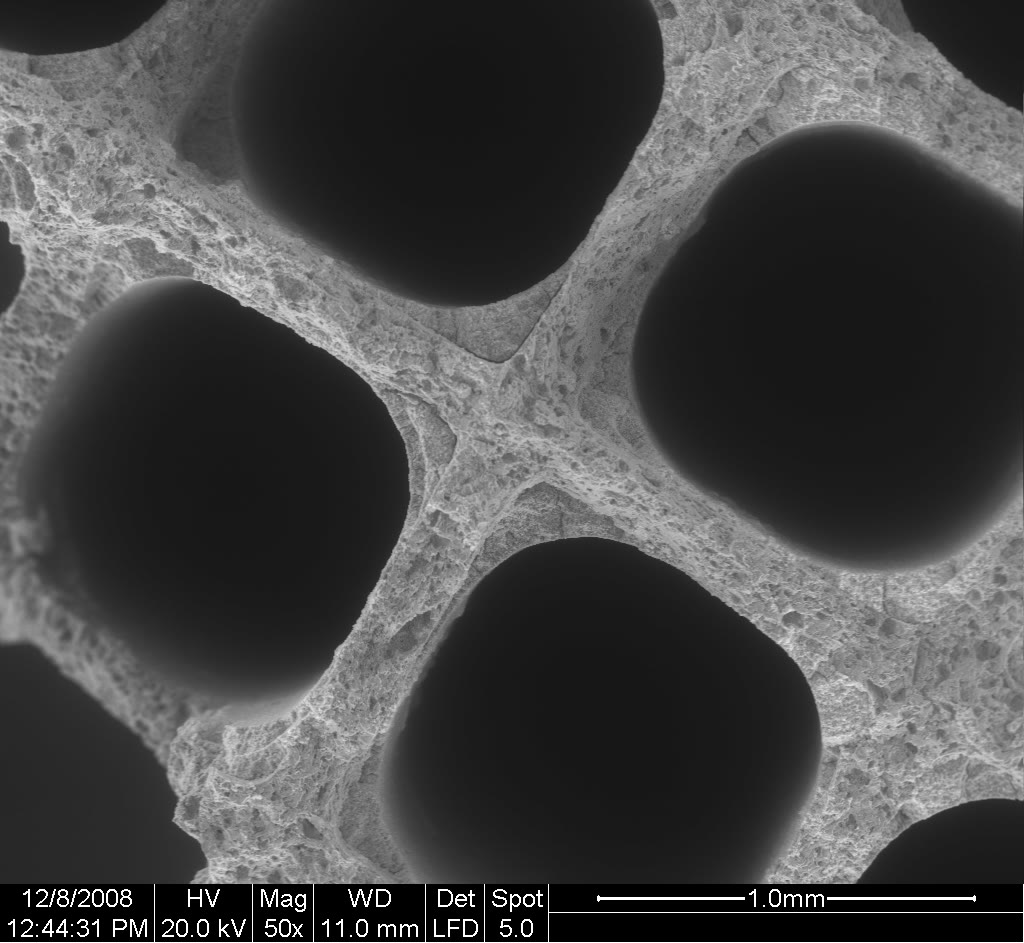
\includegraphics[width=0.48\linewidth]{images/book4/converter-sem.jpg}

{\small The ceramic honeycomb of a catalytic converter seen with a scanning
electron microscope (scale bar \qty{1.0}{mm}): square channels separated by thin
porous walls, which carry the oxide washcoat and its metal particles.}
\end{omfigure}

\section{Adsorption}

\begin{definition}[Adsorption]\label{def:b3:surfaces-catalysis:adsorption}
\emph{Adsorption}\index{adsorption} is the accumulation of molecules of a gas or
a solute on the surface of a solid or a liquid. The molecule that adsorbs is the
\emph{adsorbate}\index{adsorbate}, the solid the \emph{adsorbent}\index{adsorbent};
the reverse process is \emph{desorption}\index{desorption}.
\end{definition}

\begin{definition}[Physisorption, chemisorption]\label{def:b3:surfaces-catalysis:physi-chemi}
\emph{Physisorption}\index{physisorption} is \omterm{def:b3:surfaces-catalysis:adsorption}{adsorption} by van der Waals forces,
with enthalpies of \omterm{def:b3:surfaces-catalysis:adsorption}{adsorption} of a few tens of kilojoules per mole at most,
comparable to enthalpies of condensation, and no change of the molecule.
\emph{Chemisorption}\index{chemisorption} forms chemical bonds with the surface,
with enthalpies of about 40 to several hundred kilojoules per mole; it can
break the molecule (dissociative chemisorption) and stops at one layer.
\end{definition}

\begin{omfigure}
\begin{tikzpicture}[font=\small, >=Stealth, x=1cm, y=1cm]
  \draw[->] (0,-2.6) -- (0,1.8) node[anchor=south] {energy};
  \draw[->] (0,0) -- (8.0,0) node[anchor=south east] {distance from the surface};
  \draw[omDef, thick] plot[smooth, tension=0.7] coordinates {(1.6,1.6) (2.2,-0.25) (2.8,-0.62) (3.6,-0.35) (5.0,-0.08) (7.5,0)};
  \draw[omThm, thick] plot[smooth, tension=0.6] coordinates {(0.45,1.6) (0.8,-1.2) (1.2,-2.2) (1.7,-1.6) (2.35,-0.15) (2.9,0.9) (3.5,1.5)};
  \node[omDef, anchor=north west, font=\scriptsize] at (3.4,-0.4) {physisorbed \ce{H2} (precursor)};
  \node[omThm, anchor=west, font=\scriptsize] at (1.75,-1.9) {chemisorbed 2 H};
  \node[omThm, anchor=west, font=\scriptsize, align=left] at (3.55,1.45) {towards $\mathrm{H} + \mathrm{H}$\\ far from the surface};
  \fill (2.3,-0.2) circle (1.5pt);
  \node[font=\scriptsize] (cr) at (1.25,0.55) {crossing};
  \draw[black!60] (cr.south east) -- (2.27,-0.15);
\end{tikzpicture}

{\small Potential energy of a hydrogen molecule approaching a metal surface
(schematic). The molecule first falls into the shallow \omterm{def:b3:surfaces-catalysis:physi-chemi}{physisorption} well;
where this curve crosses the curve of two separately bonded H atoms, it can
dissociate into the deep \omterm{def:b3:surfaces-catalysis:physi-chemi}{chemisorption} well. If the crossing lies above zero,
dissociative \omterm{def:b3:surfaces-catalysis:physi-chemi}{chemisorption} is activated.}
\end{omfigure}

The surfaces of metal particles expose mostly the densest faces of the fcc
lattice, (111) and (100). On them an \omterm{def:b3:surfaces-catalysis:adsorption}{adsorbate} can sit on top of one atom
(atop), between two (bridge) or in a hollow between three or four, and the
binding energy differs from site to site.

\begin{omfigure}
\begin{tikzpicture}[font=\scriptsize]
  % fcc(111): hexagonal layer, spacing 0.6 cm
  \foreach \i in {0,...,5}{\foreach \j in {0,...,4}{
    \shade[ball color=black!25] ({0.6*\i+0.3*\j},{0.52*\j}) circle (0.29);}}
  \fill[omThm] (1.2+0.3*1,0.52) circle (0.07);
  \fill[omDef] ({0.6*2+0.3*2+0.3},{0.52*2}) circle (0.07);
  \fill[black] ({0.6*3+0.3*2+0.3},{0.52*2+0.17}) circle (0.07);
  \fill[black!60!green] ({0.6*1+0.3*3+0.3},{0.52*3-0.17}) circle (0.07);
  \node[anchor=north] at (2.1,-0.45) {fcc(111)};
  % fcc(100): square layer
  \begin{scope}[xshift=5.6cm]
  \foreach \i in {0,...,4}{\foreach \j in {0,...,4}{
    \shade[ball color=black!25] ({0.6*\i},{0.6*\j}) circle (0.29);}}
  \fill[omThm] (1.2,1.2) circle (0.07);
  \fill[omDef] (1.5,1.8) circle (0.07);
  \fill[black] (2.1,0.9) circle (0.07);
  \node[anchor=north] at (1.2,-0.45) {fcc(100)};
  \end{scope}
  \node[anchor=west, align=left] at (9.0,1.6) {\textcolor{omThm}{$\bullet$} atop\\ \textcolor{omDef}{$\bullet$} bridge\\
    $\bullet$ hollow (3- or 4-fold)\\ \textcolor{black!60!green}{$\bullet$} second 3-fold hollow (111)};
\end{tikzpicture}

{\small Top views of the two densest faces of a face-centred cubic metal, with
the \omterm{def:b3:surfaces-catalysis:adsorption}{adsorption} sites: atop one atom, bridging two, and in the hollows between
three atoms on (111) (two kinds, above an atom of the second layer or not) or
four atoms on (100).}
\end{omfigure}

\begin{definition}[Fractional coverage, monolayer]\label{def:b3:surfaces-catalysis:coverage}
The \emph{fractional coverage}\index{fractional coverage} $\theta$ of a surface is the
fraction of its \omterm{def:b3:surfaces-catalysis:adsorption}{adsorption} sites that are occupied. A
\emph{monolayer}\index{monolayer} is a single complete layer of \omterm{def:b3:surfaces-catalysis:adsorption}{adsorbate}, $\theta = 1$.
\end{definition}

\section{Isotherms}

\begin{theorem}[Langmuir isotherm]\label{thm:b3:surfaces-catalysis:langmuir}
If a surface has identical, independent sites, each holding one molecule, the
coverage at equilibrium with a gas at pressure $p$ is
\[
  \theta = \frac{Kp}{1 + Kp},
\]
where $K$, the \omterm{def:b3:surfaces-catalysis:adsorption}{adsorption} equilibrium constant, depends only on the
temperature. This is the \emph{Langmuir isotherm}\index{Langmuir isotherm}.
\end{theorem}

\begin{proof}
Kinetic proof. Molecules adsorb on the free sites at the rate $k_ap(1 - \theta)N$ ($N$
sites) and desorb at the rate $k_d\theta N$. At equilibrium the two are equal: $\theta/(1 - \theta)
= (k_a/k_d)p$, which rearranges to the result with $K = k_a/k_d$.

Statistical proof. $M$ molecules on $N$ sites can be arranged in $N!/(M!(N - M)!)$ ways,
each adsorbed molecule having an internal partition function $q_{\mathrm s}$ (its
vibrations against the surface and its binding energy). With Stirling's formula
the chemical potential of the adsorbed molecules is $\mu_{\mathrm s} = -kT\ln\bigl(q_{\mathrm s}\frac{1 - \theta}{\theta}\bigr)$;
that of the ideal gas is $\mu_{\mathrm g} = \mu_{\mathrm g}^\circ + kT\ln(p/p^\circ)$. Equilibrium, $\mu_{\mathrm s} = \mu_{\mathrm g}$, gives
$\theta/(1 - \theta) = q_{\mathrm s}\eu^{\mu_{\mathrm g}^\circ/kT}p/p^\circ$: the same law, with $K$ written in terms of
partition functions.
\end{proof}

At low pressure $\theta \approx Kp$ (Henry's regime); at high pressure $\theta \to 1$. The
coverage is one half at $p = 1/K$.

\begin{proposition}[Dissociative adsorption]\label{prop:b3:surfaces-catalysis:dissociative}
For a diatomic gas that dissociates on two sites, $\mathrm{H_2} + 2\,{*} \to 2\,\mathrm{H}{*}$ (${*}$: a free site),
\[
  \theta = \frac{(Kp)^{1/2}}{1 + (Kp)^{1/2}},
\]
so that $\theta \propto \sqrt p$ at low pressure.
\end{proposition}

\begin{proof}
\omterm{def:b3:surfaces-catalysis:adsorption}{Adsorption} needs two free sites, at the rate $k_ap(1 - \theta)^2$; \omterm{def:b3:surfaces-catalysis:adsorption}{desorption} needs two
adsorbed atoms to recombine, at the rate $k_d\theta^2$. Equality gives $\theta/(1 - \theta) =
(Kp)^{1/2}$.
\end{proof}

\begin{proposition}[Competitive adsorption]\label{prop:b3:surfaces-catalysis:competitive}
Two gases A and B competing for the same sites cover them with
\[
  \theta_{\mathrm A} = \frac{K_{\mathrm A}p_{\mathrm A}}{1 + K_{\mathrm A}p_{\mathrm A} + K_{\mathrm B}p_{\mathrm B}}, \qquad
  \theta_{\mathrm B} = \frac{K_{\mathrm B}p_{\mathrm B}}{1 + K_{\mathrm A}p_{\mathrm A} + K_{\mathrm B}p_{\mathrm B}} .
\]
\end{proposition}

\begin{proof}
For each gas, $k_{a,\mathrm A}p_{\mathrm A}(1 - \theta_{\mathrm A} - \theta_{\mathrm B}) = k_{d,\mathrm A}\theta_{\mathrm A}$ and likewise for B. Hence
$\theta_{\mathrm A} = K_{\mathrm A}p_{\mathrm A}\theta_\ast$ and $\theta_{\mathrm B} = K_{\mathrm B}p_{\mathrm B}\theta_\ast$ with $\theta_\ast = 1 - \theta_{\mathrm A} - \theta_{\mathrm B}$ the free fraction; adding,
$1 - \theta_\ast = \theta_\ast(K_{\mathrm A}p_{\mathrm A} + K_{\mathrm B}p_{\mathrm B})$.
\end{proof}

\begin{definition}[Isosteric enthalpy of adsorption]\label{def:b3:surfaces-catalysis:isosteric}
The \emph{isosteric enthalpy of adsorption}\index{isosteric enthalpy of
adsorption} $\Delta_{\mathrm{ads}}H$ is the molar enthalpy of \omterm{def:b3:surfaces-catalysis:adsorption}{adsorption} at a fixed coverage,
obtained from the pressures that give the same coverage at different
temperatures.
\end{definition}

\begin{proposition}[Isosteric enthalpy]\label{prop:b3:surfaces-catalysis:isosteric}
At constant coverage,
\[
  \Bigl(\frac{\partial\ln p}{\partial T}\Bigr)_\theta = -\frac{\Delta_{\mathrm{ads}}H}{RT^2} .
\]
\end{proposition}

\begin{proof}
At constant $\theta$, $Kp$ is constant (for a Langmuir surface; in general the same
argument holds with the equilibrium constant at that coverage), so $\ln p =
\text{const} - \ln K$. By the van 't Hoff equation, $\dd\ln K/\dd T = \Delta_{\mathrm{ads}}H/RT^2$ (with $K$
referred to a standard pressure).
\end{proof}

Since \omterm{def:b3:surfaces-catalysis:adsorption}{adsorption} is exothermic, higher temperatures need higher pressures for
the same coverage: the isotherms of the figure fall as $T$ rises.

\begin{theorem}[BET isotherm]\label{thm:b3:surfaces-catalysis:bet}
If molecules adsorb in successive layers, the first with a binding constant
characteristic of the surface and the others with the condensation equilibrium
of the liquid, the amount adsorbed at relative pressure $x = p/p^*$ ($p^*$: vapour
pressure of the liquid \omterm{def:b3:surfaces-catalysis:adsorption}{adsorbate}) is
\[
  \frac{v}{v_{\mathrm m}} = \frac{cx}{(1 - x)(1 - x + cx)},
\]
where $v_{\mathrm m}$ is the amount in a \omterm{def:b3:surfaces-catalysis:coverage}{monolayer} and $c$ a constant related to the
difference between the enthalpies of \omterm{def:b3:surfaces-catalysis:adsorption}{adsorption} in the first layer and of
condensation. This is the \emph{BET isotherm}\index{BET isotherm} (Brunauer,
Emmett and Teller).
\end{theorem}

\begin{proof}
Let $s_i$ be the fraction of the surface covered by exactly $i$ layers. The
balance of each layer, as in the Langmuir proof, gives $s_1 = cxs_0$ and $s_i =
xs_{i-1}$ for $i \ge 2$, so $s_i = cx^is_0$. The amount adsorbed is $v/v_{\mathrm m} =
\sum_iis_i/\sum_is_i$. With $\sum_{i\ge1}x^i = x/(1 - x)$ and $\sum_{i\ge1}ix^i = x/(1 - x)^2$:
\[
  \frac{v}{v_{\mathrm m}} = \frac{cs_0\,x/(1 - x)^2}{s_0[1 + cx/(1 - x)]} = \frac{cx}{(1 - x)(1 - x + cx)} .
\]
\end{proof}

Rearranged, $\dfrac{x}{v(1 - x)} = \dfrac{1}{v_{\mathrm m}c} + \dfrac{c - 1}{v_{\mathrm m}c}\,x$: a straight line whose slope and
intercept give $v_{\mathrm m}$ and $c$, usually valid for $0.05 < x < 0.30$.

\begin{definition}[Specific surface area]\label{def:b3:surfaces-catalysis:surface-area}
The \emph{specific surface area}\index{specific surface area} of a solid is its
surface area per unit mass, including the walls of its pores.
\end{definition}

\begin{method}[Specific surface area from a nitrogen isotherm]\label{met:b3:surfaces-catalysis:bet-area}
\begin{enumerate}
  \item Degas the sample under vacuum while heating; cool it in liquid nitrogen
        (\qty{77}{K}).
  \item Measure the volume of nitrogen adsorbed (reduced to standard conditions)
        at relative pressures between 0.05 and 0.30.
  \item Plot $x/(v(1 - x))$ against $x$; from slope and intercept,
        $v_{\mathrm m} = 1/(\text{slope} + \text{intercept})$ and $c = 1 + \text{slope}/\text{intercept}$.
  \item Area $= n_{\mathrm m}N_Aa_{\mathrm m}$, with $n_{\mathrm m}$ the amount in the \omterm{def:b3:surfaces-catalysis:coverage}{monolayer} and $a_{\mathrm m} = \qty{0.162}{nm^2}$
        the conventional area of an adsorbed nitrogen molecule.
\end{enumerate}
\end{method}

\begin{omfigure}
\begin{tikzpicture}
\begin{axis}[name=la, width=0.31\linewidth, height=5.0cm, xmin=0, xmax=100, ymin=0, ymax=1.05,
  axis lines=left, xlabel={$p$ / kPa}, ylabel={$\theta$}, tick label style={font=\small},
  label style={font=\small}, title={\small Langmuir}]
\addplot[omDef, thick] table[x=p_kPa, y=T300] {figdata/out/bachelor-3-langmuir-bet-langmuir.dat};
\addplot[omThm, thick] table[x=p_kPa, y=T350] {figdata/out/bachelor-3-langmuir-bet-langmuir.dat};
\node[font=\scriptsize, omDef, anchor=south east] at (axis cs:98,0.92) {\qty{300}{K}};
\node[font=\scriptsize, omThm, anchor=north east] at (axis cs:98,0.45) {\qty{350}{K}};
\end{axis}
\begin{axis}[name=be, at={(la.east)}, anchor=west, xshift=1.9cm, width=0.31\linewidth, height=5.0cm,
  xmin=0, xmax=0.9, ymin=0, ymax=200, axis lines=left, xlabel={$p/p^*$},
  ylabel={$v$ / \unit{cm^3.g^{-1}}}, tick label style={font=\small}, label style={font=\small},
  title={\small BET}]
\addplot[black, thick] table[x=x, y=v] {figdata/out/bachelor-3-langmuir-bet-bet.dat};
\addplot[only marks, mark=*, mark size=1.4pt, omDef] table[x=x, y=v] {figdata/out/bachelor-3-langmuir-bet-data.dat};
\draw[black!40, dashed] (axis cs:0,45) -- (axis cs:0.9,45);
\node[font=\scriptsize, anchor=south east] at (axis cs:0.88,45) {$v_{\mathrm m}$};
\end{axis}
\begin{axis}[at={(be.east)}, anchor=west, xshift=2.1cm, width=0.31\linewidth, height=5.0cm,
  xmin=0, xmax=0.35, ymin=0, ymax=0.0085, axis lines=left, xlabel={$x = p/p^*$},
  ylabel={$x/(v(1 - x))$}, tick label style={font=\small}, label style={font=\small},
  scaled y ticks=false, yticklabel style={/pgf/number format/fixed, /pgf/number format/precision=3},
  title={\small BET plot}]
\addplot[black, thin] table[x=x, y=y] {figdata/out/bachelor-3-langmuir-bet-line.dat};
\addplot[only marks, mark=*, mark size=1.4pt, omDef] table[x=x, y=y] {figdata/out/bachelor-3-langmuir-bet-data.dat};
\end{axis}
\end{tikzpicture}

{\small Left: \omterm{thm:b3:surfaces-catalysis:langmuir}{Langmuir isotherms} of a model \omterm{def:b3:surfaces-catalysis:physi-chemi}{chemisorption} ($\Delta_{\mathrm{ads}}H = \qty{-40}{kJ/mol}$) at
two temperatures. Middle: a \omterm{thm:b3:surfaces-catalysis:bet}{BET isotherm} (model, $v_{\mathrm m} = \qty{45}{cm^3.g^{-1}}$, $c = 120$), with the
points of the weekend problem; the layers pile up and the amount diverges near
$p = p^*$, where the gas condenses. Right: the linear BET plot of the same points.}
\end{omfigure}

\section{Kinetics of surface reactions}

\begin{definition}[Langmuir--Hinshelwood and Eley--Rideal mechanisms]\label{def:b3:surfaces-catalysis:mechanisms}
In the \emph{Langmuir--Hinshelwood mechanism}\index{Langmuir--Hinshelwood
mechanism} both reactants are adsorbed and react on the surface; in the
\emph{Eley--Rideal mechanism}\index{Eley--Rideal mechanism} an adsorbed reactant
reacts with a molecule arriving from the gas.
\end{definition}

\begin{proposition}[Langmuir--Hinshelwood rate]\label{prop:b3:surfaces-catalysis:lh-rate}
If \omterm{def:b3:surfaces-catalysis:adsorption}{adsorption} equilibria are fast and the surface reaction of adsorbed A and B
is rate-determining,
\[
  r = k\theta_{\mathrm A}\theta_{\mathrm B} = \frac{kK_{\mathrm A}p_{\mathrm A}K_{\mathrm B}p_{\mathrm B}}{(1 + K_{\mathrm A}p_{\mathrm A} + K_{\mathrm B}p_{\mathrm B})^2},
\]
which, at fixed $p_{\mathrm B}$, is largest when $K_{\mathrm A}p_{\mathrm A} = 1 + K_{\mathrm B}p_{\mathrm B}$ and then falls as A crowds B off the
surface.
\end{proposition}

\begin{proof}
The coverages are those of \cref{prop:b3:surfaces-catalysis:competitive}. With $u =
K_{\mathrm A}p_{\mathrm A}$ and $a = 1 + K_{\mathrm B}p_{\mathrm B}$, $r \propto u/(a + u)^2$, whose derivative $(a - u)/(a + u)^3$ vanishes at
$u = a$.
\end{proof}

\begin{proposition}[Eley--Rideal rate]\label{prop:b3:surfaces-catalysis:er-rate}
If adsorbed A reacts with gaseous B,
\[
  r = k\theta_{\mathrm A}p_{\mathrm B} = \frac{kK_{\mathrm A}p_{\mathrm A}p_{\mathrm B}}{1 + K_{\mathrm A}p_{\mathrm A}},
\]
which grows with $p_{\mathrm A}$ to a plateau, without a maximum.
\end{proposition}

\begin{proof}
B does not compete for the sites: $\theta_{\mathrm A}$ is the Langmuir coverage of A alone, and the
rate is proportional to it and to the collision rate of B with the surface,
proportional to $p_{\mathrm B}$.
\end{proof}

\begin{method}[LH or ER from the pressure dependence]\label{met:b3:surfaces-catalysis:mechanism-from-rate}
\begin{enumerate}
  \item Measure the rate against the pressure of each reactant, the other held
        fixed.
  \item A maximum, then a decline (negative order at high pressure):
        Langmuir--Hinshelwood, the reactant inhibiting by occupying the sites.
  \item A rise to a plateau in one reactant and first order in the other at all
        pressures: Eley--Rideal.
  \item Confirm with isotope labelling or surface spectroscopy; most catalytic
        reactions turn out to be of the Langmuir--Hinshelwood type.
\end{enumerate}
\end{method}

\begin{omfigure}
\begin{tikzpicture}
\begin{axis}[width=0.6\linewidth, height=5.4cm, xmin=0, xmax=10, ymin=0, ymax=0.3,
  axis lines=left, xlabel={$p_{\mathrm A}$ (reduced)}, ylabel={rate (reduced)},
  tick label style={font=\small}, label style={font=\small},
  legend style={font=\scriptsize, draw=none, at={(1.03,0.98)}, anchor=north west}, legend cell align=left]
\addplot[omDef!50, thick] table[x=pA, y=pB05] {figdata/out/bachelor-3-surface-rates.dat};
\addplot[omDef, thick] table[x=pA, y=pB1] {figdata/out/bachelor-3-surface-rates.dat};
\addplot[black, thick] table[x=pA, y=pB3] {figdata/out/bachelor-3-surface-rates.dat};
\addplot[omThm, thick, dashed] table[x=pA, y=ER] {figdata/out/bachelor-3-surface-rates.dat};
\legend{{LH, $p_{\mathrm B} = 0.5$}, {LH, $p_{\mathrm B} = 1$}, {LH, $p_{\mathrm B} = 3$}, {ER ($\times\frac14$)}}
\end{axis}
\end{tikzpicture}

{\small Rates of a bimolecular surface reaction against the pressure of A
(reduced units, $K_{\mathrm A} = K_{\mathrm B} = 1$). Langmuir--Hinshelwood: each curve peaks at $K_{\mathrm A}p_{\mathrm A} =
1 + K_{\mathrm B}p_{\mathrm B}$, then falls as A displaces B. Eley--Rideal (dashed, scaled): a plateau.}
\end{omfigure}

\begin{proposition}[Apparent activation energy]\label{prop:b3:surfaces-catalysis:apparent-ea}
For a unimolecular surface reaction with Langmuir \omterm{def:b3:surfaces-catalysis:adsorption}{adsorption}, $r = k\theta = kKp/(1 + Kp)$.
At low coverage the measured activation energy is $E_{a,\mathrm{app}} = E_a + \Delta_{\mathrm{ads}}H$; at
high coverage it is $E_a$.
\end{proposition}

\begin{proof}
At low coverage $r \approx kKp$, so $\dd\ln r/\dd T = \dd\ln k/\dd T + \dd\ln K/\dd T = (E_a + \Delta_{\mathrm{ads}}H)/RT^2$.
At high coverage $\theta \approx 1$ and $r \approx k$.
\end{proof}

Since $\Delta_{\mathrm{ads}}H < 0$, a reaction on a sparsely covered surface looks easier than its
true barrier: raising the temperature speeds up the surface step but empties
the surface.

\begin{definition}[Sabatier principle, volcano plot]\label{def:b3:surfaces-catalysis:sabatier}
The \emph{Sabatier principle}\index{Sabatier principle} states that the best
catalyst binds the reactants neither too weakly (they do not adsorb or
activate) nor too strongly (the products do not leave and block the sites). A
\emph{volcano plot}\index{volcano plot} of the activity of a series of
catalysts against a binding energy has a maximum at intermediate binding.
\end{definition}

\begin{omfigure}
\begin{tikzpicture}[font=\small, >=Stealth]
  \draw[->] (0,0) -- (7.2,0) node[anchor=north east] {binding strength of the adsorbate};
  \draw[->] (0,0) -- (0,3.6) node[anchor=south] {activity};
  \draw[omDef, very thick] (0.4,0.3) -- (3.4,3.0) -- (6.6,0.4);
  \node[anchor=south, align=center, font=\scriptsize] at (1.35,2.0) {binds too weakly:\\ reactants not\\ activated};
  \node[anchor=south, align=center, font=\scriptsize] at (5.9,2.0) {binds too strongly:\\ products block\\ the sites};
  \node[anchor=south, font=\scriptsize] at (3.4,3.05) {best catalyst};
\end{tikzpicture}

{\small A \omterm{def:b3:surfaces-catalysis:sabatier}{volcano plot} (qualitative): the activity of a series of catalysts
against the strength with which they bind a key intermediate.}
\end{omfigure}

\section{Industrial catalysts}

\begin{definition}[Catalyst design]\label{def:b3:surfaces-catalysis:catalyst-design}
A \emph{catalyst support}\index{catalyst support} is a porous, high-area solid
(alumina, silica, carbon) that carries small particles of the active phase. A
\emph{promoter}\index{promoter} is an additive, inactive alone, that raises the
activity, selectivity or stability. A \emph{catalyst poison}\index{catalyst
poison} is a substance that binds strongly to the \omterm{def:b3:complex-kinetics:enzyme}{active sites} and blocks them.
The \emph{metal dispersion}\index{metal dispersion} $D$ is the fraction of the metal
atoms that lie on the surface. \emph{Sintering}\index{sintering} is the growth of
the particles at high temperature, which lowers the dispersion.
\end{definition}

\begin{method}[Dispersion and particle size from hydrogen chemisorption]\label{met:b3:surfaces-catalysis:dispersion}
\begin{enumerate}
  \item Reduce the catalyst in hydrogen, evacuate, and measure the volume of \ce{H2}
        chemisorbed (reduced to standard conditions) on the metal; the
        support adsorbs none.
  \item Assume one H atom per surface metal atom: $D = n_{\ce{H}}/n_{\text{metal}}$.
  \item For spheres of diameter $d$, $D = 6(v_{\mathrm{at}}/a_{\mathrm{at}})/d$, with $v_{\mathrm{at}}$ the volume per atom in the
        bulk and $a_{\mathrm{at}}$ the area per surface atom; hence $d = 6v_{\mathrm{at}}/(a_{\mathrm{at}}D)$.
\end{enumerate}
\end{method}

Ammonia synthesis, $\ce{N2 + 3 H2 <=> 2 NH3}$, runs at about 400 to \qty{500}{\celsius} and 100 to
\qty{300}{bar} over iron promoted with potassium oxide and alumina: the alumina keeps
the iron crystallites from \omterm{def:b3:surfaces-catalysis:catalyst-design}{sintering}, the potassium raises the activity. The
rate-determining step is the dissociative \omterm{def:b3:surfaces-catalysis:physi-chemi}{chemisorption} of \ce{N2}, whose triple
bond is the hardest to break. Some 150 million tonnes of nitrogen a year are
fixed in this way.
% ledger: nh3:world-2024
The oxidation of \ce{SO2} to \ce{SO3}, on vanadium(V) oxide promoted
with potassium sulfate, is the key step of sulfuric acid manufacture.

The three-way converter of petrol engines oxidises CO and hydrocarbons and
reduces nitrogen oxides at the same time, on platinum and palladium (oxidation)
and rhodium (reduction of NO), dispersed on alumina with cerium oxide, which
stores and releases oxygen. It works only in a narrow window around the
stoichiometric air--fuel ratio: with excess air the NO is not reduced, with
excess fuel the CO is not oxidised; an oxygen sensor in the exhaust keeps the
engine in the window. Lead from leaded fuel poisons the metal, which is one
reason leaded petrol disappeared. Zeolites, crystalline aluminosilicates with
pores of molecular size and acidic sites, crack the large molecules of heavy
oil fractions into petrol and admit only molecules that fit their channels.

\begin{omfigure}
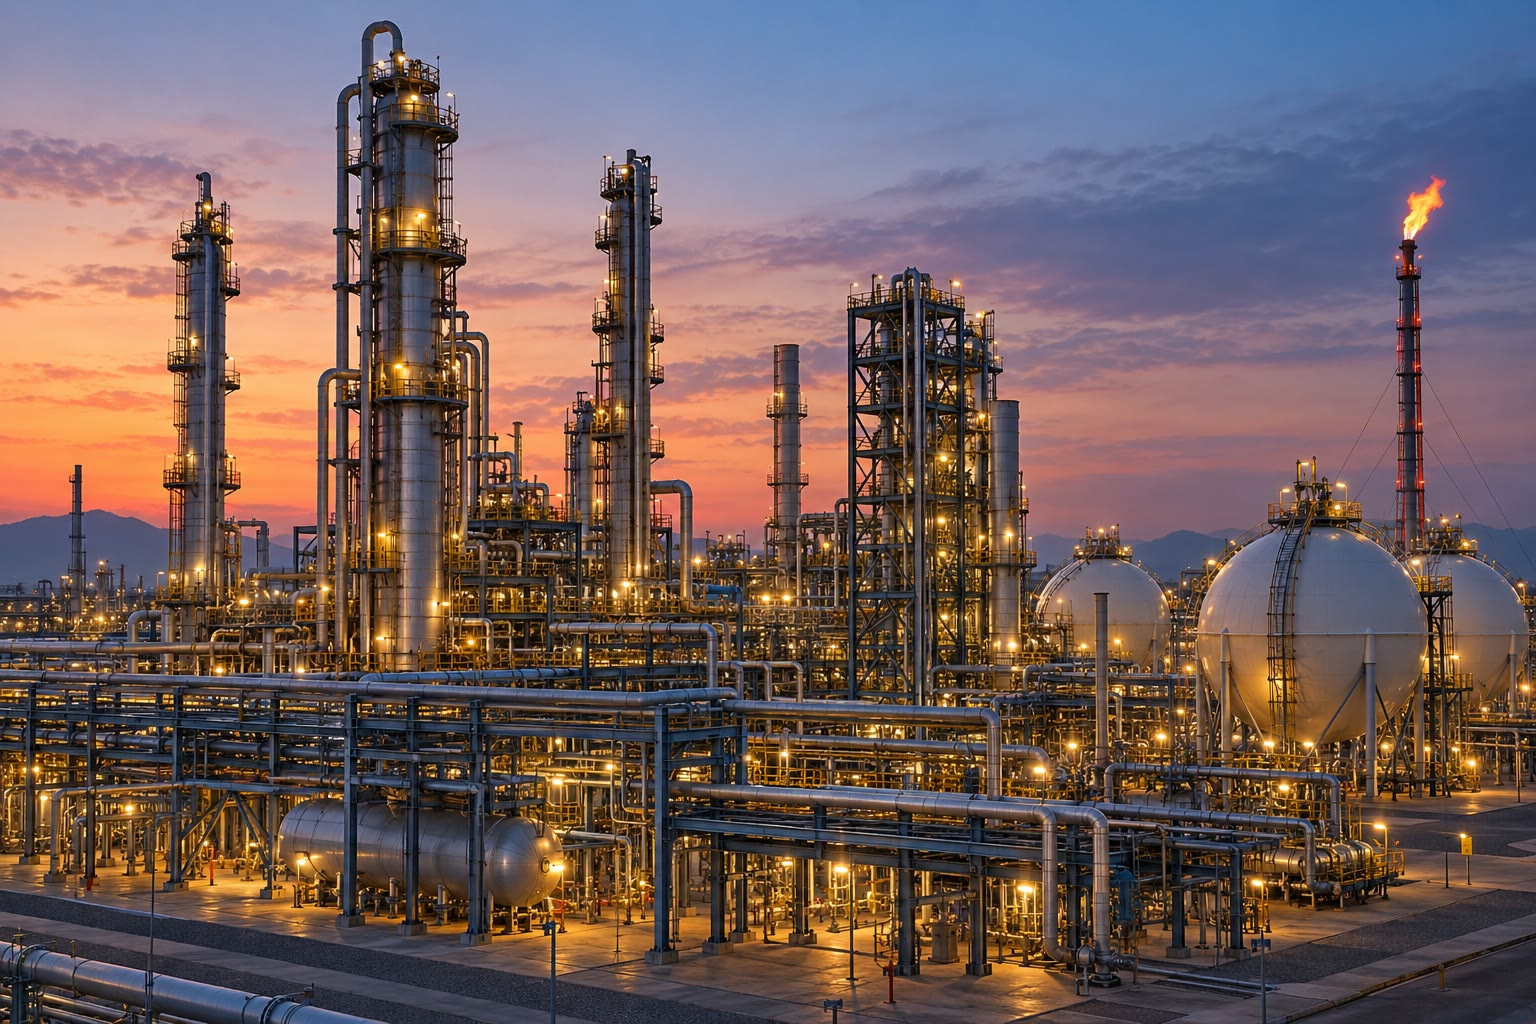
\includegraphics[width=0.6\linewidth]{images/book4/ai/b3-16-ammonia-plant.jpg}

{\small An ammonia synthesis plant. The reactor at its heart holds tonnes of
promoted iron catalyst; most of the plant prepares the hydrogen and recycles
the unconverted gas.}
\end{omfigure}

\section{Looking at surfaces}

\begin{definition}[Thermal desorption spectroscopy]\label{def:b3:surfaces-catalysis:tpd}
\emph{Thermal desorption spectroscopy}\index{thermal desorption spectroscopy}
heats a surface carrying an \omterm{def:b3:surfaces-catalysis:adsorption}{adsorbate} at a constant rate and records the
desorbing gas with a mass spectrometer; each binding state gives a peak, whose
temperature increases with its \omterm{def:b3:surfaces-catalysis:adsorption}{desorption} activation energy.
\end{definition}

The position of a \omterm{def:b3:surfaces-catalysis:adsorption}{desorption} peak gives the \omterm{def:b3:surfaces-catalysis:adsorption}{desorption} energy (for first-order
\omterm{def:b3:surfaces-catalysis:adsorption}{desorption}, $E_d \approx RT_{\mathrm p}[\ln(\nu T_{\mathrm p}/\beta) - 3.64]$ with $\beta$ the heating rate and $\nu \approx \qty{e13}{s^{-1}}$,
admitted), its area the amount adsorbed. Photoelectron spectroscopy with
X-rays (XPS) measures the binding energies of core electrons of the surface
atoms, which identify the elements and their oxidation states in the first few
nanometres. The scanning \omterm{def:b3:quantum-model-systems:tunnelling}{tunnelling} microscope moves a sharp tip a few tenths
of a nanometre above a conducting surface; the \omterm{def:b3:quantum-model-systems:tunnelling}{tunnelling} current
(\cref{ch:b3:quantum-model-systems}) falls by about an order of magnitude for
each \qty{0.1}{nm} of extra distance, so that keeping it constant while scanning
maps the surface atom by atom.

\begin{inthelab}[A BET measurement]
About \qty{0.2}{g} of sample is weighed into a glass tube with a bulb, degassed
for hours under vacuum at 150 to \qty{300}{\celsius}, weighed again, and mounted on the
instrument, the bulb immersed in a dewar of liquid nitrogen. The instrument
admits nitrogen in small doses and measures the equilibrium pressure after each,
deducing the amount adsorbed from the gas balance; the dead volume of the tube
is measured with helium, which does not adsorb.
\end{inthelab}

\begin{safety}{\ghs[0.7cm]{GHS06}\ghs[0.7cm]{GHS07}\ghs[0.7cm]{GHS08}\ghs[0.7cm]{GHS09}}
% ledger: ghs4:V2O5, ghs4:Ni
Reduced metal catalysts (finely divided nickel, palladium or platinum on a
support, freshly reduced in hydrogen) can ignite on contact with air: they are
handled under inert gas and passivated before storage. Nickel is a skin
sensitiser and a suspected carcinogen; vanadium(V) oxide is toxic if inhaled
and swallowed and may cause cancer. Catalyst powders are weighed in a
ventilated enclosure.
\end{safety}

\begin{history}[Langmuir and the ammonia catalyst]
Irving Langmuir, working on light bulbs in an industrial laboratory, derived
his isotherm in 1916--1918 from the idea that adsorbed gases form a layer one
molecule thick, and received the 1932 Nobel Prize in Chemistry for his surface
chemistry. A few years earlier, Alwin Mittasch had organised the search for a
practical ammonia catalyst: thousands of compositions were tested in small
high-pressure reactors before the promoted iron catalyst, still in use, was
chosen. It was one of the first systematic catalyst screenings.
\end{history}

\section{Exercises}

\begin{exercise}[$\star$]\label{exo:b3:surfaces-catalysis:1}
A gas covers 40\,\% of a Langmuir surface at \qty{2.0}{kPa}. Compute $K$ and the coverage at
\qty{10}{kPa}.
\end{exercise}

\begin{exercise}[$\star$]\label{exo:b3:surfaces-catalysis:2}
Two \omterm{def:b3:surfaces-catalysis:adsorption}{adsorption} enthalpies are measured on a metal: $-20$ and \qty{-150}{kJ/mol}. Which
is \omterm{def:b3:surfaces-catalysis:physi-chemi}{physisorption}, which \omterm{def:b3:surfaces-catalysis:physi-chemi}{chemisorption}? Which could be dissociative?
\end{exercise}

\begin{exercise}[$\star$]\label{exo:b3:surfaces-catalysis:3}
Count, per surface atom, the atop, bridge and hollow sites of a (100) face and of
a (111) face of an fcc metal.
\end{exercise}

\begin{exercise}[$\star$]\label{exo:b3:surfaces-catalysis:4}
A catalyst converts \qty{3.0e-6}{mol} of reactant per gram per second and carries
\qty{1.5e-5}{mol} of surface sites per gram. Compute the turnover frequency.
\end{exercise}

\begin{exercise}[$\star\star$]\label{exo:b3:surfaces-catalysis:5}
Hydrogen adsorbs dissociatively with $\theta = 0.10$ at \qty{1.0}{kPa}. Compute $\theta$ at \qty{4.0}{kPa}.
\end{exercise}

\begin{exercise}[$\star\star$]\label{exo:b3:surfaces-catalysis:6}
CO ($K = \qty{10}{kPa^{-1}}$) and \ce{O2} ($K = \qty{0.5}{kPa^{-1}}$, non-dissociative in this simple model)
compete for the sites of a platinum surface at 1.0 and \qty{5.0}{kPa}. Compute the two
coverages and comment on the CO oxidation rate.
\end{exercise}

\begin{exercise}[$\star\star$]\label{exo:b3:surfaces-catalysis:7}
A coverage reached at \qty{1.0}{kPa} at \qty{300}{K} needs \qty{8.0}{kPa} at \qty{350}{K}. Compute the \omterm{def:b3:surfaces-catalysis:isosteric}{isosteric
enthalpy of adsorption}.
\end{exercise}

\begin{exercise}[$\star\star$]\label{exo:b3:surfaces-catalysis:8}
% ledger: sa:N2.am, const:Vm1, const:NA
An activated carbon has $v_{\mathrm m} = \qty{120}{cm^3.g^{-1}}$ (standard conditions, 273.15 K and
\qty{101.325}{kPa}). Compute its BET area.
\end{exercise}

\begin{exercise}[$\star\star$]\label{exo:b3:surfaces-catalysis:9}
The rate of $\ce{2 CO + O2 -> 2 CO2}$ on platinum rises, passes a maximum and falls as $p(\ce{CO})$
increases at fixed $p(\ce{O2})$. Which mechanism does this indicate, and why does CO
inhibit the reaction?
\end{exercise}

\begin{exercise}[$\star\star\star$]\label{exo:b3:surfaces-catalysis:10}
A surface reaction has a true activation energy of \qty{100}{kJ/mol}; the reactant has
$\Delta_{\mathrm{ads}}H = \qty{-60}{kJ/mol}$. What activation energy is measured at low and at high
coverage? Sketch $\ln r$ against $1/T$ over a wide range.
\end{exercise}

\begin{exercise}[$\star\star\star$]\label{exo:b3:surfaces-catalysis:11}
Sulfur adsorbs on a nickel catalyst with a coverage of 0.10 (sulfur atoms per
surface Ni), each sulfur atom blocking four sites. What fraction of the activity
remains for a reaction needing one free site? Two adjacent free sites (assume
randomly placed blocked sites)?
\end{exercise}

\begin{exercise}[$\star\star\star$]\label{exo:b3:surfaces-catalysis:12}
For ammonia synthesis, three metals bind atomic nitrogen with enthalpies of
$-150$, $-250$ and \qty{-400}{kJ/mol} (data of the exercise). Using the \omterm{def:b3:surfaces-catalysis:sabatier}{Sabatier
principle}, which is likely the best catalyst, and what limits the other two?
\end{exercise}

\section{Problem: Measuring a Catalyst}

\begin{problem}[{Weekend problem --- measuring a catalyst: the BET area of a
supported platinum catalyst, its metal dispersion and particle size from
hydrogen chemisorption, and the turnover frequency of a hydrogenation}]
\label{pb:b3:surfaces-catalysis:1}
% ledger: sa:N2.am, lat:Pt, aw:Pt, const:Vm1, const:NA
A catalyst contains 1.00\,\% by mass of platinum on alumina. Data of the problem:
nitrogen isotherm at \qty{77}{K} (volumes at standard conditions, 273.15 K and
\qty{101.325}{kPa}, per gram):
\begin{center}\small
\begin{tabular}{lcccccc}
\hline
$x = p/p^*$ & 0.05 & 0.10 & 0.15 & 0.20 & 0.25 & 0.30 \\
$v$ / \unit{cm^3.g^{-1}} & 41.2 & 46.1 & 51.1 & 54.1 & 58.9 & 62.9 \\ \hline
\end{tabular}
\end{center}
\ce{H2} chemisorbed on the platinum: \qty{0.205}{cm^3} per gram of catalyst. A hydrogenation
runs at \qty{2.0e-5}{mol} per gram of catalyst per second. Platinum: $M = \qty{195.08}{g/mol}$, fcc,
$a = \qty{392.3}{pm}$; molar volume of a gas at standard conditions \qty{22414}{cm^3/mol};
$a_{\mathrm m}(\ce{N2}) = \qty{0.162}{nm^2}$.

\medskip\noindent\textbf{Part I --- The BET plot.}
\begin{enumerate}
  \item Why is the isotherm measured at \qty{77}{K}?
  \item Why are only relative pressures between 0.05 and 0.30 used?
  \item Compute $x/(v(1 - x))$ for each point.
  \item The least-squares line has slope \num{0.02205} and intercept \num{0.000180} (in
        \unit{g.cm^{-3}}). Deduce $v_{\mathrm m}$.
  \item Deduce $c$. What does a large $c$ mean?
  \item Why is the intercept so poorly determined, and does it matter for $v_{\mathrm m}$?
\end{enumerate}

\medskip\noindent\textbf{Part II --- The area.}
\begin{enumerate}[resume]
  \item Compute the amount of nitrogen in the \omterm{def:b3:surfaces-catalysis:coverage}{monolayer} per gram.
  \item Compute the \omterm{def:b3:surfaces-catalysis:surface-area}{specific surface area}.
  \item Which part of the solid provides almost all of this area?
  \item Why does the BET method fail for microporous solids such as zeolites?
\end{enumerate}

\medskip\noindent\textbf{Part III --- Dispersion and particle size.}
\begin{enumerate}[resume]
  \item Compute the amount of H atoms chemisorbed per gram.
  \item Compute the amount of platinum per gram.
  \item Deduce the dispersion.
  \item Compute the volume per Pt atom in the bulk.
  \item The area per surface atom, averaged over the (111), (100) and (110)
        faces, is \qty{0.0807}{nm^2}. Check the (111) value, $\frac{\sqrt3}{4}a^2$.
  \item Show that for spheres $d = 6v_{\mathrm{at}}/(a_{\mathrm{at}}D)$.
  \item Compute the mean particle diameter.
  \item Which assumptions limit this result?
\end{enumerate}

\medskip\noindent\textbf{Part IV --- Activity.}
\begin{enumerate}[resume]
  \item Compute the turnover frequency per surface Pt atom.
  \item Compute the rate per gram of platinum.
  \item If the particles sintered to \qty{10}{nm} at constant turnover frequency, by what
        factor would the rate per gram fall?
  \item What would a turnover frequency that changes with particle size reveal?
  \item Why are catalysts compared by turnover frequency rather than rate per
        gram?
  \item State the result: the mean diameter of the platinum particles.
\end{enumerate}
\end{problem}
